%!TEX root = ../dokumentation.tex


\chapter{Sudoku}
Nachdem in der Einleitung schon kurz auf das Spielfeld eines Sudokus und die Regeln eingegangen wurde, werden beides in diesem Kapitel noch einmal ausführlicher behandelt. Es wird auch auf Elemente des Spielfelds eingegangen, die relevant sind für die Strategien und wie das Spielfeld in dem Programm aufgebaut ist und eine einheitliche Identifikation definiert. Im letzten Abschnitt wird das Prinzip der Strategien, um ein Sudoku lösen zu können, behandelt. Da für die Strategien und den \textbf{Sudoku Solver} die Lösungshilfe der Kandidaten-Notation eine wichtige Rolle spielt, wird darauf in einem weiteren Unterkapitel eingegangen und die Funktion und Bedeutung erklärt.



\section{Spielfeld Aufteilung}
Zunächst wird die Aufteilung des Spielfelds erläutert und die Units vorgestellt. Jede Unit bekommt einen eindeutigen Identitiver, auf den im weiteren Verlauf der Arbeit referenziert werden kann.

Das Spielfeld, auf dem ein Sudoku gespielt wird, besteht aus einem 9x9 Gitter und damit aus 81 einzelnen Zellen. Diese Gitter wird weiterhin in je neun Zeilen, Spalten und 3x3 Blöcke aufgeteilt. Jede Aufteilung, weiterhin auch Unit genannt, besteht immer aus neun Zellen. Damit kann ein Sudoku also nochmal in 27 verschiedene Units aufgeteilt werden. Wie diese Units aussehen, wird im Folgenden gezeigt.

\subsection{Zeile}
Eine Zeile in einem Sudokuspielfeld sind Zellen, die horizontal zueinander ausgerichtet sind. In der Abbildung \ref{fig:SudokugitterZeile} wurde die oberste Zeile beispielhaft markiert.
\begin{figure}[htbp]
	\centering
	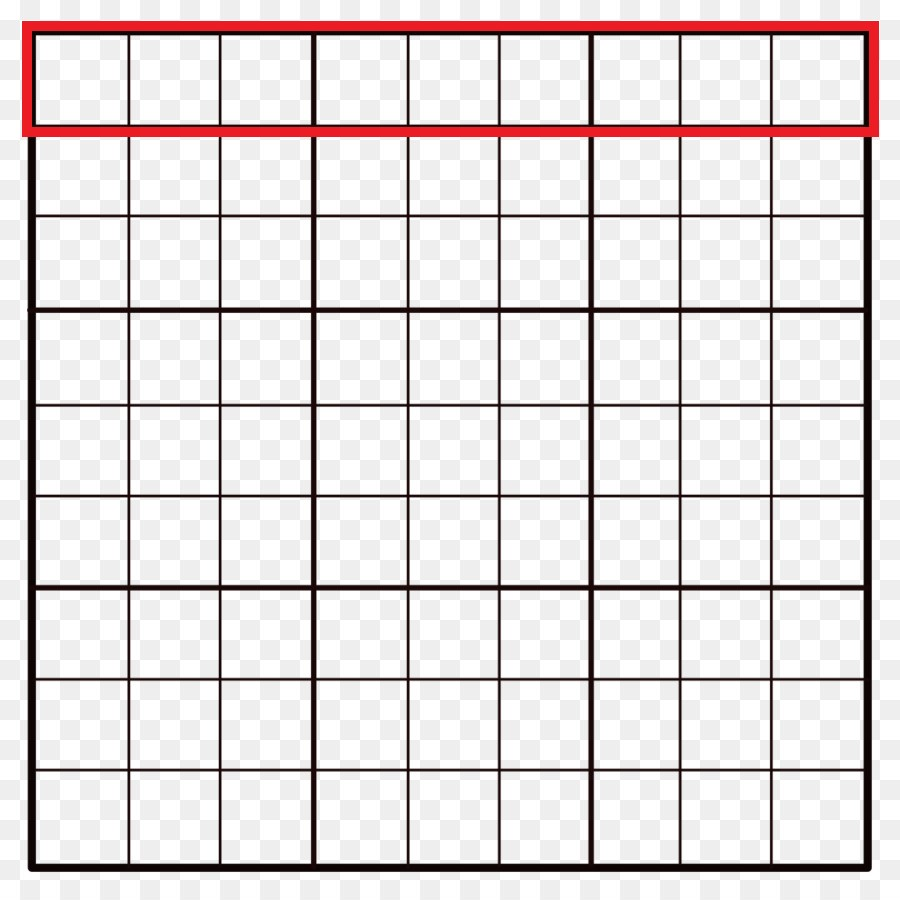
\includegraphics[width=0.3\textwidth]{images/sudokugitterZeile.jpg}
	\caption{Darstellung des Sudokugitters mit der Markierung einer Zeile}
	\label{fig:SudokugitterZeile}
\end{figure}
Auf die Zeilen wird ab jetzt und im Folgenden der Arbeit mit den Zahlen 1 bis 9 referiert. 

\subsection{Spalte}
Analog zu einer Reihe sind Spalten Zellen, die vertikal zueinander ausgerichtet sind. In der Abbildung \ref{fig:SudokugitterSpalte} wurde beispielhaft die erste Spalte markiert.
\begin{figure}[htbp]
	\centering
	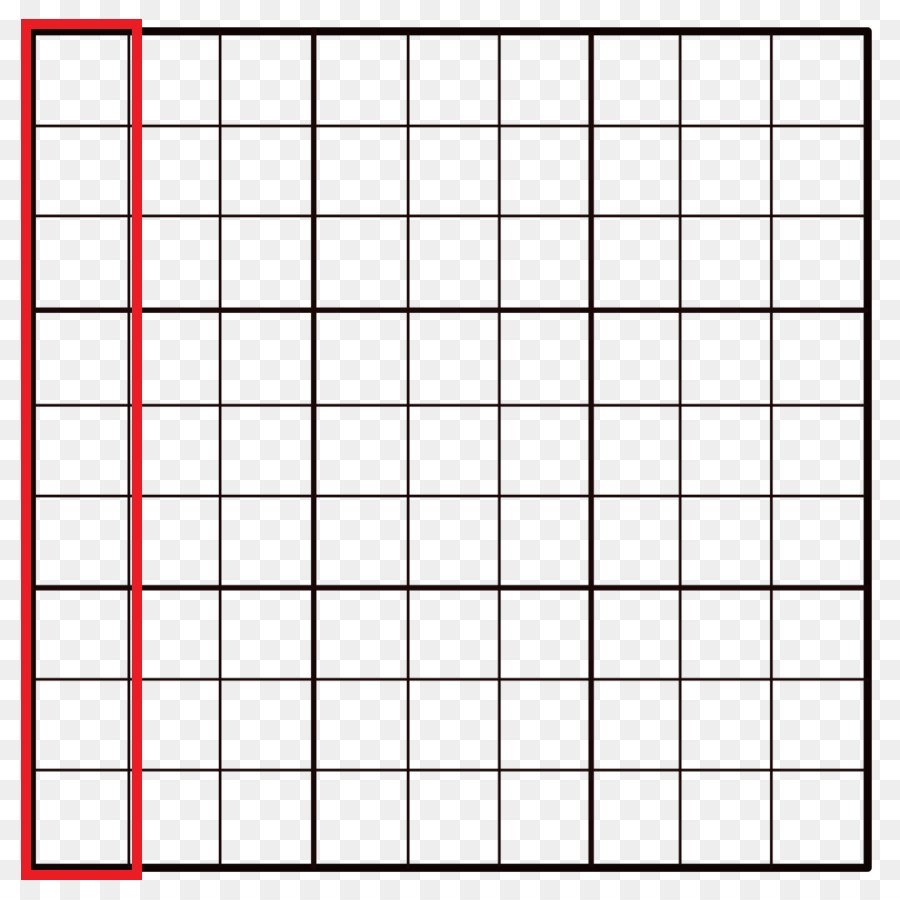
\includegraphics[width=0.3\textwidth]{images/sudokugitterSpalte.jpg}
	\caption{Darstellung des Sudokugitters mit der Markierung einer Spalte}
	\label{fig:SudokugitterSpalte}
\end{figure}
Die Spalten werden ähnlich zu den Zeilen von links nach rechts nicht mit Zahlen, sondern mit den Buchstaben A bis I beschrieben.

\subsection{Box/Block}
Boxen bestehen aus 3x3 Zellen. Die 3x3 Boxen sind im Sudokufeld so angeordnet, dass jede Zelle in genau einer Box liegt und, dass es neun Boxen geben kann. In der Abbildung \ref{fig:SudokugitterBox} wurde eine Box markiert. Wie zu erkennen ist, sind die Boxen auch im Frontend durch dickere Linien voneinander abgegrenzt. 
\begin{figure}[htbp]
	\centering
	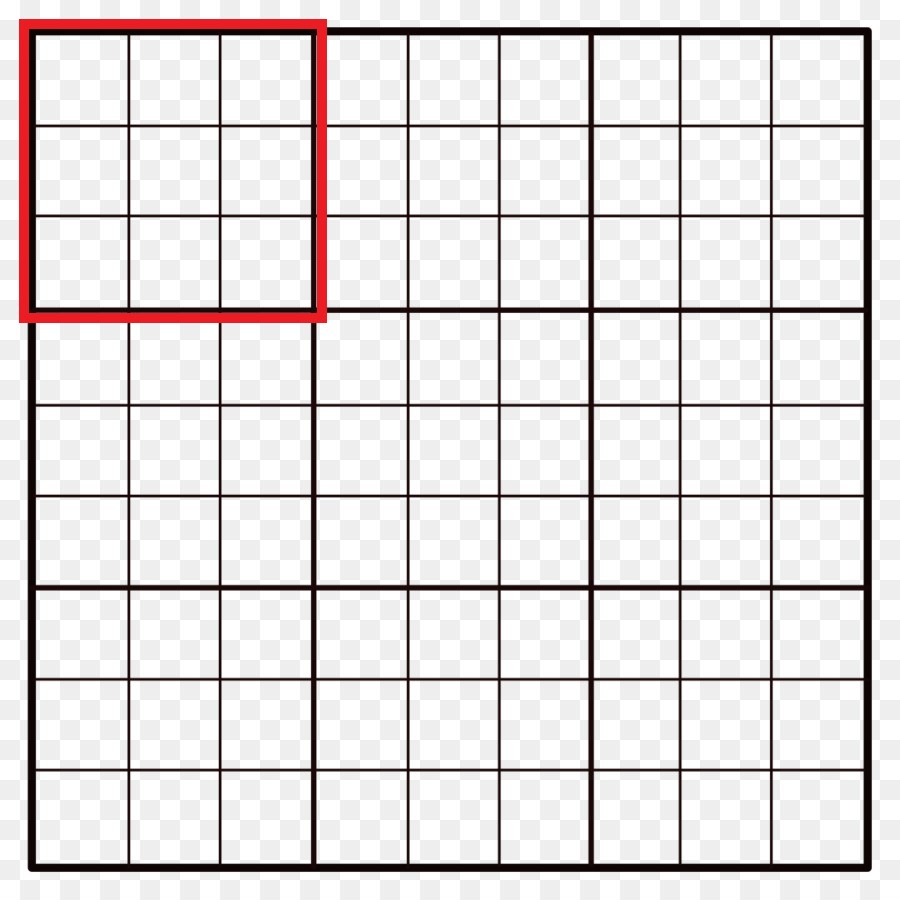
\includegraphics[width=0.3\textwidth]{images/sudokugitterBox.jpg}
	\caption{Darstellung des Sudokugitters mit der Aufteilung in 9 Boxen}
	\label{fig:SudokugitterBox}
\end{figure}
Blöcke werden durch römische Zahlen identifiziert. Dabei wird erst von links nach rechts und von dann von oben nach unten mit I bis IX nummeriert.

\section{Regeln}
Nachdem die Abgrenzungen der Units und damit die Aufteilung des Spielfelds definiert wurde, werden die Regeln auf Basis des jetzigen Wissensstand nochmals genauer erläutert.

Die Regeln ergeben sich durch einfache Bedingungen, wenn man die Aufteilung des Spielfeldes kennt. In jeder Zeile, Spalte und Box dürfen und müssen die Zahlen von eins bis neun nur einmal vorkommen.

Am Ende kommen die Zahlen von eins bis neun also jeweils neunmal auf dem gesamten Sudokugitter vor, ohne dass sie sich gegenseitig sehen, also sich keine Zahl doppelt in einer Zeile, Spalte oder Box befindet.

Damit man das Sudokugitter ausfüllen kann und es nur eine mögliche Lösung gibt, sind zu Spielbeginn einige Ziffern vorgegeben. Mithilfe dieser Ziffern ist es möglich, mit den gerade erklärten Regeln das ganze Sudokugitter durch Logik und Deduktionen zu füllen. \cite{sudopedia_2022}

\section{Strategie}
In diesem Abschnitt wird die Bedeutung von Strategien im Sinne des Lösens eines Sudokus beschrieben. Es werden zwei verschiedene Arten von Strategien angesprochen. In diesem Sinne wird das Hilfsmittel der Kandidaten-Notation gebraucht und daher erläutert.

Um ein Sudoku zu lösen, können verschiedene Strategien eingesetzt werden. Das Ziel einer Strategie ist es hierbei eine passende Zahl in das Sudoku einzufügen oder mögliche Kandidaten zu eliminieren. Es gibt zwei grundlegende Strategien, um Zahlen direkt einzufügen: den Hidden Single und den Naked Single. Beide Strategien können oft intuitiv und ohne eine große Erklärung gefunden und umgesetzt werden. Weitere leichte Strategien wie ein Hidden Double oder ein Naked Double, bei denen Kandidaten eliminiert werden können, sind mithilfe der Kandidaten-Notation leicht gefunden.

Insgesamt gibt es über 30 gebräuchliche Strategien, die zur Unterstützung bei schweren Sudokus angewendet werden können. Oftmals sind anspruchsvollere Strategien für das menschliche Auge schwer zu entdecken. Wichtig bei diesen komplexeren Strategien ist eine gewissenhafte Ausführung der Kandidaten-Notation.\cite{martin}

\subsection{Lösungshilfen: Kandidaten-Notation}
Kandidaten sind Zahlen in einer Zelle des Sudokugitters, die, mit dem aktuellen Informationsstand, als feste Zahl noch infrage kommen. Das Problem liegt dabei, dass meistens mehrere Zahlen in eine Zelle können. Kandidaten können durch das Eintragen von weiteren Zahlen oder das Anwenden von Strategien eliminiert werden. Wenn man dabei jede Zelle einzeln betrachtet, geben die Kandidaten keinen weiteren Nutzen. Wenn die Kandidaten jedoch über mehrerer Zellen in Bezug zueinander angeschaut werden, lassen sich Zusammenhänge erkennen. Die meisten Strategien basieren auf diesen Zusammenhängen. 

Sobald eine Zahl eingetragen wird, müssen die Kandidaten aktualisiert werden. Wenn eine Zahl eingetragen wird, kann jeder gleichwertiger Kandidat, der diese Zahl sieht, gestrichen werden.
